\documentclass[tikz,border=2pt]{standalone}
\usepackage{amsmath,amssymb}
\usepackage{tikz}
\usetikzlibrary{arrows.meta}

\begin{document}
% A norm measures length: scaling a vector scales its norm (homogeneity), and the diagonal of
% the parallelogram is never longer than the two sides together (triangle inequality).
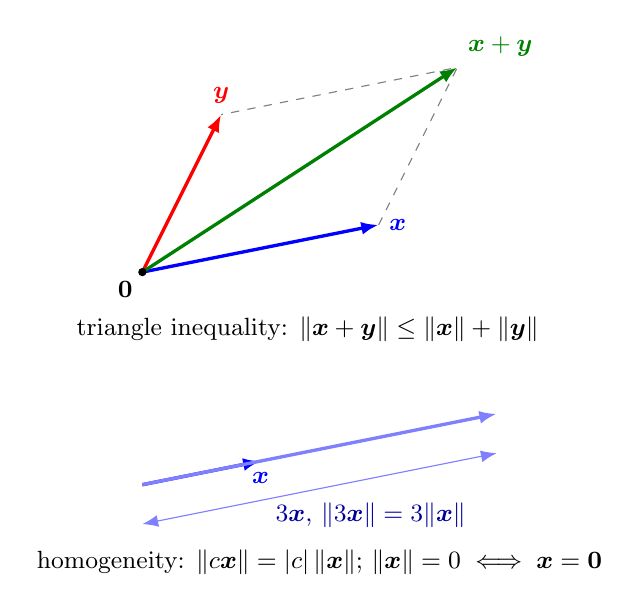
\begin{tikzpicture}[scale=1.0, every node/.style={font=\small}, >={Latex[length=2.2mm]}]
	\draw[->, blue, very thick] (0,0) -- (3,0.6) node[right] {$\boldsymbol{x}$};
	\draw[->, red, very thick] (0,0) -- (1,2) node[above] {$\boldsymbol{y}$};
	\draw[->, green!50!black, very thick] (0,0) -- (4,2.6) node[above right] {$\boldsymbol{x}+\boldsymbol{y}$};
	\draw[gray, dashed] (3,0.6) -- (4,2.6) -- (1,2);
	\fill (0,0) circle (1.5pt) node[below left] {$\boldsymbol{0}$};
	\node[anchor=north] at (2.1,-0.45) {triangle inequality: $\|\boldsymbol{x}+\boldsymbol{y}\|\le\|\boldsymbol{x}\|+\|\boldsymbol{y}\|$};
	\begin{scope}[yshift=-2.7cm]
		\draw[->, blue, very thick] (0,0) -- (1.5,0.3) node[below] {$\boldsymbol{x}$};
		\draw[->, blue!50, very thick] (0,0) -- (4.5,0.9);
		\draw[blue!50, {Latex[length=2mm]}-{Latex[length=2mm]}] (0,-0.5) -- (4.5,0.4);
		\node[blue!60!black, anchor=north] at (2.9,-0.1) {$3\boldsymbol{x}$, $\|3\boldsymbol{x}\|=3\|\boldsymbol{x}\|$};
		\node[anchor=north] at (2.25,-0.7) {homogeneity: $\|c\boldsymbol{x}\|=|c|\,\|\boldsymbol{x}\|$; $\|\boldsymbol{x}\|=0\iff\boldsymbol{x}=\boldsymbol{0}$};
	\end{scope}
\end{tikzpicture}
\end{document}
